% usar Tex Live e lualatex
% usar minted v2.9
% custom compiler argument: -shell-escape


\documentclass{../class/IFSCprova}

\usepackage[pdftex,
            pdfauthor={Prof. Jackson Lago, Dr.},
            pdftitle={Introdução ao Python: notas de aula},
            pdfkeywords={python},
            pdfcreator={LuaLaTex, Biber},
            pdfborder={0 0 0}]{hyperref}
\usepackage{import}

\definecolor{primary}{RGB}{137, 197, 63}
\definecolor{secondary}{RGB}{234, 32, 38}
\definecolor{bgcsv}{rgb}{0.95,0.95,0.85}

\newcommand{\plotscale}{0.51}
\newcommand{\todo}{To be done!}

\newcommand{\0}{_{_{\! n\!}}}
\newcommand{\1}{_{_{\! n\text{-}\!\>\!1\!}}}
\newcommand{\2}{_{_{\! n-\!2\!}}}
\newcommand{\questao}[2][]{\addtocounter{section}{1}\section*{Questão \thesection: #1} \addcontentsline{toc}{section}{Questão \thesection: #1} \input{#2}}

\newcommand{\myfrac}[3][0pt]{\genfrac{}{}{}{}{\raisebox{#1}{$#2$}}{\raisebox{-#1}{$#3$}}}

\definecolor{civ}{rgb}{1.0,0.4,0.0}

%-----------------------------------------------------------------------------------------------------------------------
\autor{Jackson Lago, Dr. Eng.}
\disciplina{NVP68300 -- Programação Aplicada a Sistemas de Energia}
\curso{Mestrado Profissional em Sistemas de Energia}
\titulo{Avaliação}

%-----------------------------------------------------------------------------------------------------------------------
\begin{document}

%
\maketitle

\vspace{10mm}
\noindent
    \textbf{Orientações gerais:}
\emph{
    \begin{enumerate}[label=\roman*)]
        %\item   Confirme o recebimento desse arquivo respondendo o e--mail com o número encontrado no canto
        %superior direito dessa página;
        \item   A interpretação das questões faz parte da avaliação;
        \item   O tempo destinado à resolução das questões também será considerado na avaliação;
        %\item   Resolva a prova e envie apenas os arquivos {\texttt{.m}}, nomeados como indicado em cada questão, para
        %        {\texttt{\href{mailto:jackson.lago@ifsc.edu.br}{jackson.lago@ifsc.edu.br}}} impreterivelmente
        %        até as \textbf{21h}.
        %        Respostas enviadas depois desse horário não serão consideradas;
        \item   Resolva a prova nomeando os arquivos \texttt{.py} conforme indicado em cada questão.
        Após concluir, reúna todos os arquivos \texttt{.py} gerados em uma única pasta, compacte-a e nomeie o arquivo compactado com seu primeiro e último nome (\texttt{fulano\_tal.zip}).
        Faça o upload dessa pasta compactada na tarefa aberta no SIGAA impreterivelmente até às \textbf{21:30}.
        O sistema está configurado para não aceitar respostas enviadas após esse horário, o que resultará em nota \textbf{zero} e, consequentemente, na reprovação do candidato;
        \item   Todos os arquivos \texttt{.py} necessários para a execução dos algoritmos devem ser entregues;
        \item   Não envie arquivos que não tenham sido criados por você.
        Arquivos de saída e figuras geradas não devem ser enviados, pois devem ser produzidos automaticamente pelos seus algoritmos;
        \item   Na primeira linha de cada arquivo \texttt{.py}, inclua um comentário com seu nome completo e a qual questão da avaliação o arquivo está vinculado (Ex: \texttt{\# Fulano de Tal, Q2});
        \item   Parte ou todas as questões poderão ser corrigidas automaticamente por um algoritmo que verifica se as soluções atendem aos requisitos especificados nos respectivos enunciados.
        Portanto, atente-se à implementação correta das funções e scripts, bem como à nomenclatura dos arquivos, nomes das funções, variáveis de retorno e argumentos, conforme indicado em cada questão;
        %\item   Todas as questões têm peso igual;
        \item   Para aprovação, é necessário atingir nota \textbf{maior ou igual} a 6,0;
        \item   A prova é individual, sendo permitida apenas a consulta ao documento \texttt{python\_tutorial.pdf} (disponibilizado no SIGAA) e ao seu caderno de anotações pessoal;
        \item   Cópias, mesmo que parciais, configuram plágio.
        Em caso de plágio, será atribuída nota \textbf{zero} à avaliação de todos os envolvidos, o que resultará na reprovação do(s) candidato(s) e, consequentemente, no desligamento do programa de mestrado.
    \end{enumerate}
}

    \vspace{2mm}

    \newpage

    \section*{Q1: \texttt{harmonicas.py}}

Nas análises de qualidade de energia em sistemas elétricos trifásicos, é comum modelar distorções nos sinais de tensão e
corrente por meio da decomposição harmônica.
Essa técnica representa sinais periódicos como a soma de componentes senoidais de diferentes frequências, permitindo
identificar e quantificar distúrbios como a distorção harmônica total e a presença de harmônicas específicas que podem
afetar o desempenho de equipamentos e a eficiência do sistema

Além disso, as componentes harmônicas ímpares podem ser classificadas em três categorias, com base na sua ordem $h$
(um número inteiro positivo e ímpar), conforme sua relação com o número de fases do sistema (geralmente três):


\begin{itemize}
\item Sequência zero: quando $h$ é múltiplo de 3, ou seja, $h \mod 3 = 0$.
\item Sequência positiva: quando $h \mod 3 = 1$.
\item Sequência negativa: quando $h \mod 3 = 2$.
\end{itemize}

Implemente uma função que receba uma lista de inteiros positivos representando ordens harmônicas e os
classifique nas três categorias descritas acima.
A função deve retornar uma tupla com três listas:
\begin{itemize}
\item A primeira contendo os valores de sequência zero;
\item A segunda contendo os valores de sequência positiva; e
\item A terceira contendo os valores de sequência negativa.
\end{itemize}


Se não houver valores em alguma categoria, a lista correspondente deve ser vazia.

Se houver valores pares, ignore-os, e não os inclua em nenhuma das três categorias.

Assuma que o argumento é uma lista de inteiros positivos (sem necessitar de uma validação disso interna a sua função).

\begin{minted}{custompython}
def classifica_harmonicas(hs: list) -> tuple[list, list, list]:
    # seu código aqui


# Exemplo de uso
ordem_harmonicas = [5, 7, 9, 3, 2, 11, 13, 15, 1]

zero, pos, neg = classifica_harmonicas(ordem_harmonicas)
print(f"componentes harmônicas de sequência zero: {zero}")
print(f"componentes harmônicas de sequência positiva: {pos}")
print(f"componentes harmônicas de sequência negativa: {neg}")
\end{minted}

Resultado esperado:
\begin{minted}{text}
componentes harmônicas de sequência zero: [9, 3, 15]
componentes harmônicas de sequência positiva: [7, 13, 1]
componentes harmônicas de sequência negativa: [5, 11]
\end{minted}

Dica: Em python, a operação matemática $\mod$ pode ser realizada pelo operador \texttt{\%}.



    \input{prova/q2}
    \input{prova/q3}
    \section*{Q4: \texttt{grafico.py}}

Escreva um script para plotar as funções
%$$
%f_1(x)=\left\{
%\begin{aligned}
%x^2 \ \ \ \  \  \ \ \ \ \ &, 0\leq x < 4 \\
%16 \ \ \ \ \ \ \ \ \ \ \ &, 4\leq x < 6 \\
%(x-10)^2 \ \ \ \ \ \ \ \ \ \ \ &, 6\leq x < 10 \\
%-(x-10)^2 \ \ \ \ \ \ \ \ \ \ \ &, 10\leq x < 14 \\
%-16 \ \ \ \ \ \ \ \ \ \ \ &, 14\leq x < 16 \\
%-(x-20)^2 \ \ \ \ \ \ \ \ \ \ \ &, 16 \leq x < 20 \\
%\end{aligned}
%\right.
%$$

$$
g(x)=\left\{
\begin{aligned}
\dfrac{-1}{1+e^{6\cdot(x-1)}}+1 \  \ \ \ \ &, 0\leq x < 5 \\
\dfrac{-1}{1+e^{6\cdot(9-x)}}+1 \  \ \ \ \ &, 5\leq x < 10 \\
\dfrac{-1}{1+e^{6\cdot(11-x)}} \  \ \ \ \ &, 10\leq x < 15 \\
\dfrac{-1}{1+e^{6\cdot(x-19)}} \  \ \ \ \ &, 15\leq x < 20 \\
\end{aligned}
\right.
$$
e
$$
f(x)=\dfrac{\sqrt{6}}{2} \sin\left( \dfrac{\pi}{10}x\right)
$$
para o intervalo $0\leq x\leq 20$.

Além de plotar as duas funções sobrepostas, o script deve ainda adicionar grade, identificação dos eixos e legendas (replicar a figura abaixo).
\begin{figure}[htbp]
	\centering
		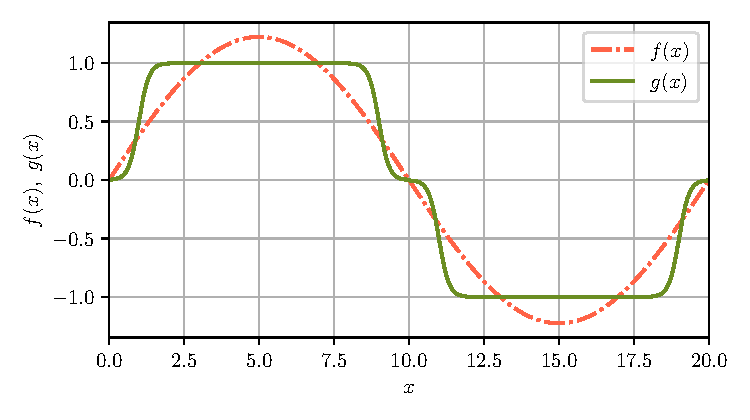
\includegraphics[scale=0.75]{figs/q4}
\end{figure}



\end{document}